\chapter{Design}
In this section we present the design of our software application MusicDAO. MusicDAO is a mobile music streaming and discovery app, with peer-to-peer payment to artists in the form of donations and subscriptions. The MusicDAO is fully decentralized by design. This means there are no intermediaries, third parties or proprietary servers needed. All users of the app form a community to share audio tracks and transfer money. Any user can join this community, publish their musical works and receive money from its listeners. With the goal of distributing power in the music industry, every peer in the network will have the same rights and access to the same functions.

\section{Phone-to-phone connectivity}
Mobile phones have the largest share of any type of device using music streaming services. If the software that we design and implement runs well on a network consisting of only mobile devices, we can conclude that it will run well on better hardware (such as PCs) as well. For these reasons, we design our system to work on mobile phones only.

\section{Release model}
\label{sec:release-model}
A Release is an object describing a list of tracks that are published by a clearly identifiable artist or group of artists. For example, a Release can represent a single, and EP or an album. It is modeled as shown in fig. \ref{fig:release-model}. Release objects are shared between peers in the network. By discovering many of those objects, a user can see and browse through them to select a track to play. A Release object merely contains metadata of the tracks. We design the network to have a separate channel for downloading the track files. This is to enable fast discovery and
searching of Releases, as Release objects have a small byte size. 
\begin{figure}
    \minipage{0.2\textwidth}
        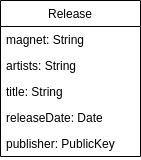
\includegraphics[width=\linewidth]{design/release-model.png}
        \caption{Release blocks structure as seen on TrustChain}
        \label{fig:release-model}
    \endminipage\hfill
    \minipage{0.3\textwidth}
        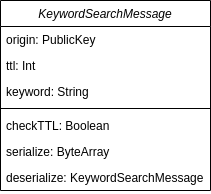
\includegraphics[width=\linewidth]{design/KeywordSearchMessage-model.png}
        \caption{KeywordSearchMessage object sent over IPv8 in MusicCommunity}
        \label{fig:keyword-search-message-model}
    \endminipage\hfill
    \minipage{0.5\textwidth}
    \endminipage
\end{figure}

\section{Identity and authenticity}
\label{sec:pki-design}
As we design a system that is fully decentralized, we cannot use a central database to record user identities. Therefore every user should generate a unique identity to be used in the network, and must be able to give proof of this identity. We use a public key infrastructure (PKI) which achieve these goals. Every user stores their private and public key on their device, and only share their public key. The keypair has a mathematical property that allows verification of messages that are signed with a private key. By comparing the public key of a peer with their signed message, anyone can verify the authenticity of the message.

In the context of MusicDAO we use this PKI to proof ownership of Release objects. All Release objects are signed using the owner's private key and the signature is added to the object. Any user receiving this object can verify its authenticity.

\section{Distributed storage}
Central to our system is sharing downloading and storage of audio files and Release objects (see \ref{sec:release-model}). To design a system which has no middlemen or regulators for publishing Releases, and has no central control, a distributed storage system is required. This storage system should have the following properties: immutability (data cannot be tampered with), resiliency (data should be available as long as users want it) and rigorous duplication (all objects should live on multiple devices so they do not disappear when requested). Distributed ledger technology (DLT) allows for these properties, so we design our system with a DLT as a major component.

\section{Distributed downloading and uploading}
To be able to have low latency for discovering and playing music tracks, while using no central nor high-throughput servers, the network demands participants to upload content continuously. We design the app to, by default, use the network capabilities of the mobile device to upload content as much as possible. This is constrained by networking hardware, data subscription plans and other software running on the phone.

\section{Distributed search algorithm}
For searching content we use a simple distributed algorithm called XYZ (cite). Pseudocode of this algorithm is shown in fig. X. It asks peers around for content tagged with some keyword. When a peer finds a match on their local database, it sends this Release object to the original asking peer. Otherwise it forwards the query to their neighbours, after reducing the time-to-live property by 1. The messages stop being forwarded once their time-to-live property hits below 1. The structure of search messages are shown in fig. \ref{fig:keyword-search-message-model}.

\section{Direct payments without intermediaries}
As we are designing a system with no intermediaries, it should be possible to give money directly to artists. Cryptocurrency allows for peer-to-peer payments which achieve this goal, so we use this in the MusicDAO. Cryptocurrency payments will be used for two different functionalities: a user can send a donation to an artist, or a user can pay artists using a monthly subscription system. This subscription system pays artists that the user listened to, using the Artist Income Division Algorithm (see \ref{sec:aida-design}).

\subsection{Wallet}
Cryptocurrency implementations allow for private/public key-pairs which can be interpreted as a kind of wallet; the funds can only be unlocked by a holder of the private key. In the case of MusicDAO we design the app to include a wallet for every user. To receive money, every artist should share their public key to all of their listeners. To achieve this, the public key of their cryptocurrency wallet is included as a property of the Release objects (see \ref{sec:release-model}). As there are no institutions or banks involved in storing money, users will be required to keep their private key safe.

\subsection{Artist Income Division Algorithm}
\label{sec:aida-design}
To provide a stable income for artists, in the form of reoccurring payments, we design the Artist Income Division Algorithm. This algorithm calculates how periodic subscription money is split into payments to artists. The user can enable a periodic payment. This money is then divided over the artists the user listens to, in proportion to the amount of interaction with each artist. Interaction can be measured in e.g. time listened, plays or feedback in the form of likes. The details of this division is explained in the implementation section of AIDA (see X).
\todo[inline]{This sec may be removed}